% Updated in September 2016 by Huei-Yung Lin
% Updated in September 2014 by Hideo Saito
% Updated in September 2012 by In Kyu Park
% Updated in April 2002 by Antje Endemann, ...., and in September 2010 by Reinhard Klette
% Based on CVPR 07 and LNCS style, with modifications by DAF, AZ and elle 2008, AA 2010, ACCV 2010, ACCV 2012

\documentclass[runningheads]{llncs}
\usepackage{graphicx}
\usepackage{amsmath,amssymb} % define this before the line numbering.
%\usepackage{lineno}
\usepackage{color}
\usepackage{url}
\usepackage{times}
\usepackage{epsfig}
%\usepackage{url}
\usepackage{subfigure}
\usepackage{lineno}
\usepackage{setspace}
\usepackage{upgreek}
\usepackage{authblk}
\usepackage{xpatch}

%===========================================================
\begin{document}

%macro for raising the point in decimal numbers; see example in the abstract
\newcommand{\point}{
    \raise0.7ex\hbox{.}
    }

%Do   -- NOT --    use any additional macros

\pagestyle{headings}

\mainmatter

%===========================================================
\title{Patch Group based Bayesian Learning for Blind Image Denoising} % Replace with your title

\titlerunning{Patch Group based Bayesian Learning for Blind Image Denoising} % Replace with your title

\authorrunning{Jun Xu, Dongwei Ren, Lei Zhang, David Zhang}
\author{Jun Xu$^{1}$, Dongwei Ren$^{1,2}$, Lei Zhang$^{1}$\footnote{This work is supported by the HK RGC GRF grant (PolyU5313/12E).}, David Zhang$^{1}$} % Replace with your names
\institute{$^{1}$Dept. of Computing, The Hong Kong Polytechnic University, Hong Kong, China\\
$^{2}$School of Computer Science and Technology, Harbin Institute of Technology, Harbin, China}

\maketitle

%===========================================================
\begin{abstract}
Most existing image denoising methods assume to know the noise distributions, e.g., Gaussian noise, impulse noise, etc. However, in practice the noise distribution is usually unknown and is more complex, making image denoising still a challenging problem. In this paper, we propose a novel blind image denoising method under the Bayesian learning framework, which automatically performs noise inference and reconstructs the latent clean image. By utilizing the patch group (PG) based image nonlocal self-similarity prior, we model the PG variations as Mixture of Gaussians, whose parameters, including the number of components, are automatically inferred by variational Bayesian method. We then employ nonparametric Bayesian dictionary learning to extract the latent clean structures from the PG variations. The dictionaries and coefficients are automatically inferred by Gibbs sampling. The proposed method is evaluated on images with Gaussian noise, images with mixed Gaussian and impulse noise, and real noisy photographed images, in comparison with state-of-the-art denoising methods. Experimental results show that our proposed method performs consistently well on all types of noisy images in terms of both quantitative measure and visual quality, while those competing methods can only work well on the specific type of noisy images they are designed for and perform poorly on other types of noisy images. The proposed method provides a good solution to blind image denoising.
\end{abstract}

%===========================================================
\section{Introduction}
Image denoising is an important problem in image processing and computer vision. Most existing methods are designed to deal with specific types of noise, e.g., Gaussian noise, mixed Gaussian and impulse noise, etc. Gaussian noise removal is a fundamental problem and has received intensive research interests with many representative work \cite{rudin1992nonlinear,nlm,foe,ksvd,bm3d,lssc,epll,mlp}. Gaussian noise removal is not only an independent task but also can be incorporated into other tasks, e.g., the removal of mixed Gaussian and impulse noise. The 'first-impulse-then-Gaussian' strategy is commonly adopted by methods of \cite{cai2010fast,l1l0,wesnr}, which are designed specifically for mixed Gaussian and impulse noise. However, noise in real images is more complex than simple Gaussian or mixed Gaussian and impulse distribution. Besides, noise is usually unknown for existing methods. This makes image denoising still a challenging problem.

To the best of our knowledge, the study of blind image denoising can be traced back to the BLS-GSM model \cite{blsgsm}. In \cite{blsgsm}, Portilla et al. proposed to use scale mixture of Gaussian in overcomplete oriented pyramids to estimate the latent clean images. In \cite{fullyblind}, Portilla proposed to use a correlated Gaussian model for noise estimation of each wavelet subband. Based on the robust statistics theory \cite{huber2011robust}, Rabie modeled the noisy pixels as outliers, which could be removed via Lorentzian robust estimator \cite{rabie2005robust}. Liu et al. proposed to use 'noise level function' (NLF) to estimate the noise and then use Gaussian conditional random field to obtain the latent clean image \cite{Liu2008}. Recently, Gong et al. proposed an optimization based method \cite{almapg}, which models the data fitting term by weighted sum of $\ell_{1}$ and $\ell_{2}$ norms and the regularization term by sparsity prior in the wavelet transform domain. Later, Lebrun el al. proposed a multiscale denoising algorithm called 'Noise Clinic' \cite{noiseclinic} for blind image denoising task. This method generalizes the NL-Bayes \cite{nlbayes} to deal with signal and frequency dependent noise.

Despite the success of these methods, they have many limitations. On one hand, as suggested in \cite{Liu2008,noiseclinic}, Gaussian noise, assumed by \cite{fullyblind,rabie2005robust,Liu2008}, may be inflexible for more complex noise in real images. Hence, better approximation to the noise could bring better image denoising performance \cite{Liu2008,noiseclinic}. On the other hand, the method \cite{almapg} needs tune specific parameters for different types of noise. This makes the proposed method not a strictly "blind" image denoising. Based on these observations, it is still needed to design an robust and effective model for blind image denoising. Few assumption and no parameter tuning would bring extra points.

In this paper, we propose a new method for blind image denoising task. The key factor of success is to employ the Mixture of Gaussian (MoG) model to fit the patches extracted from the image. Since the noise in real image is unknown, we utilize variational Bayesian inference to determine all the parameters, including the number of components. That is, the noise is modeled by a MoG adapted to the testing image. This data driven property makes our model able to deal with blind noise. Then we employ the nonparametric Bayesian model \cite{hjort1990} to reconstruct the latent clean structures in each component. Specificly, the beta-Bernoulli process \cite{thibaux2007,paisley2009} is suitable for this task. In our proposed method, the noise in each component is assumed to be Gaussian. The parameters of the beta-Bernoulli process are automatically determined by nonparametric strategies such as the Gibbs sampling. The proposed model is tested on Gaussian noise, mixed Gaussian and impulse noise,and real noise in photographed images.

To summarize, our paper has the following contributions:
\vspace{-0.1in}
\begin{itemize}
\item We proposed a noval framework for blind image denoising problem; 
\item The proposed model is more robust on image denoising tasks than the competing methods; 
\item We demonstrated that, the performance of the Beta Process Factor Analysis (BPFA) model can be largely improved by structural clustering strategy and Non-local self similarity property;
\item We achieve comparableor even better performance on blind image denoising tasks than the competing methods.
\end{itemize}

The remainder of this paper is organized as follows. Section II introduces the related workd. Section III introduces the patch group based Mixture of Gaussian model infered by variational Bayesian method. In section IV, we will formulate the proposed PG based nonparametric Bayesian dictionary learning model. Section V summarizes the overall algorithm. In section VI, we will present the experimental results, as well as discussions, on blind image denoising tasks. Section VII concludes this paper.

%------------------------------------------------------------------------- 
\section{Related Work}
\textbf{Structural clustering} are employed by many image denoising methods. For example, both EPLL \cite{epll} and PLE \cite{ple} utilized the Mixture of Gaussian (MoG) model \cite{prml} for clustering similar patches. NCSR \cite{ncsr} utilized the k-means algorithm. The recently proposed Patch Group Prior based Denoising (PGPD) \cite{pgpd} employ the MoG model to learn the non-local self-similarity (NSS) prior of images. However, all these methods need preset the number of clusters. In \cite{bpfa}, the Beta-Bernoulli Factor Analysis (BPFA) model is further extended by nonparametric clustering processes such as Dirichlet process (DP) \cite{ferguson1973bayesian} or probit stick-breaking processes (PSBP) \cite{ren2011logistic}. However, the authors in \cite{bpfa} pointed out that, the resulting 'clustering-aided' models achieved similar performance on image denoising to the original BPFA model \cite{bpfa}. In this paper, we demonstrate that, we could indeed improve the performance of Bayesian methods on image denoising tasks, if we utilize the structural clustering strategy properly.

\textbf{Dictionary learning} is very useful for image denoising tasks. The dictionary can be chosen off-the-shelf (wavelets and curvelets) or can be learned from natural image patches. The seminal work of K-SVD \cite{ksvd} has demonstrated that dictionary learning not only can help achieves promising denoising performance, but also can be used in other image processing applications. In image denoising, dictionary learning is commonly combined with the non-local self-similarity (NSS) prior \cite{nlm,pgpd}, sparse prior \cite{bm3d,lssc,ncsr}, and low rank prior \cite{wnnm}, etc. Though work well on Gaussian noise removal, the above methods perform poorly on other types of noises, especially noise in real noisy images.
\vspace{-0.1in}
%------------------------------------------------------------------------- 
\section{Patch Group based Bayesian Learning for Structural Clustering}\label{sec2}
\subsection{Patch Group based Non-local Self Similarity Property}
Non-local self similarity (NSS) is a common image prior employed by many image restoration methods \cite{nlm,bm3d,lssc,ncsr,wnnm,pgpd}. In PGPD \cite{pgpd}, the patch group (PG) based NSS prior is learned on clean natural images for efficient image denoising. In this paper, however, we apply the PG based NSS prior directly on testing noisy images. Given a noisy image, we firstly extract image patches of size $p\times p$. Then, for each image patch, we find the $M$ most similar patches to it in a large enough local window of size $W\times W$. The similarity measurement is based on Euclidean distance, i.e., $\ell_{2}$ norm, which is commonly used in other methods \cite{bm3d,lssc,ncsr,wnnm,pgpd}. In this work, we set $p=8$, $M=6$, $W=31$. The PG is a set of similar patches $\{\mathbf{x}_{m}\}_{m=1}^{M}$, in which the $\mathbf{x}_{m}\in \mathbb{R}^{p^{2}\times1}$ is the $m$th patch vector. The group mean of this PG is $\boldsymbol{\upmu}=\frac{1}{M}\sum_{m=1}^{M}\mathbf{x}_{m}$. The $m$th group mean subtracted patch vector is $\mathbf{\overline{x}}_{m}=\mathbf{x}_{m}-\boldsymbol{\upmu}$. The $\mathbf{\overline{X}}\triangleq \{\mathbf{\overline{x}}_{m}\}$, $m=1,...,M$ is called the PG variations. In Figure \ref{fig1}, we show one example of PG, PG mean, and the PG variations after group mean subtraction.
\begin{figure}
\centering
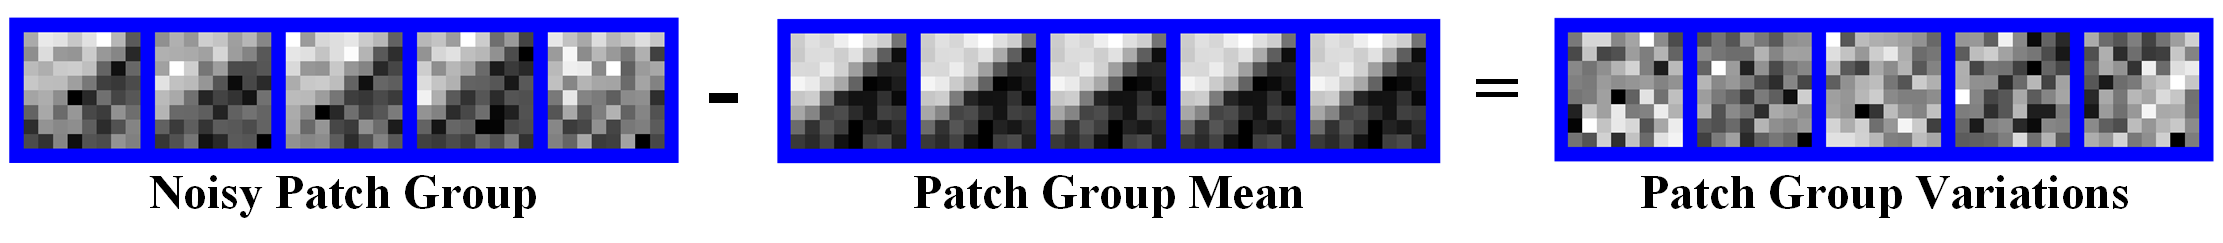
\includegraphics[width=1\textwidth]{PGResiduals2.png}
\vspace{-0.3in}
\caption{An example of PG, PG mean (duplicated by five), and PG variations after mean subtraction. The PG is from the image 'House' corrupted by Gaussian noise.}
\label{fig1}\vspace{-0.1in}
\end{figure}
The PG mean is the main structure of this PG. Here, we proposed to embed this idea into the BPFA model \cite{bpfa} and compare the performance on the Gaussian noise removal. The results are listed in Figure \ref{fig2}. When comparing the images (b) and (d), we can see that the introduce of PG based NSS prior can really boost the performance on image denoising of the BPFA model. The improvements on PSNR is nearly 0.8dB and on SSIM is nearly 0.03. In particular, the image quality in (d) is much better than that in (b). 
\vspace{-0.1in}
\begin{figure}
\centering
\subfigure{
\begin{minipage}[t]{0.19\textwidth}
\raisebox{-0.15cm}{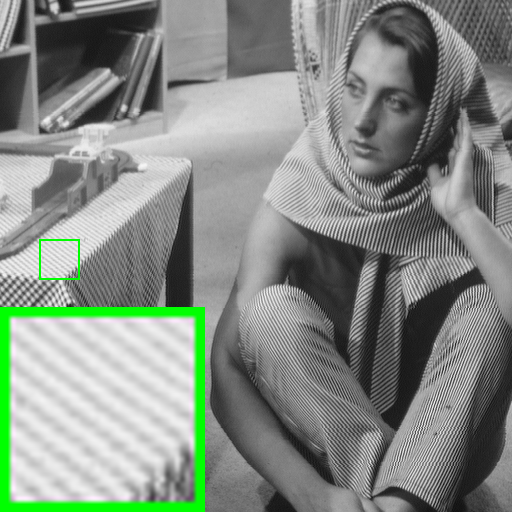
\includegraphics[width=1\textwidth]{br_Original_barbara.png}}
{\footnotesize (a) Ground Truth}
\end{minipage}
\begin{minipage}[t]{0.19\textwidth}
\centering
\raisebox{-0.15cm}{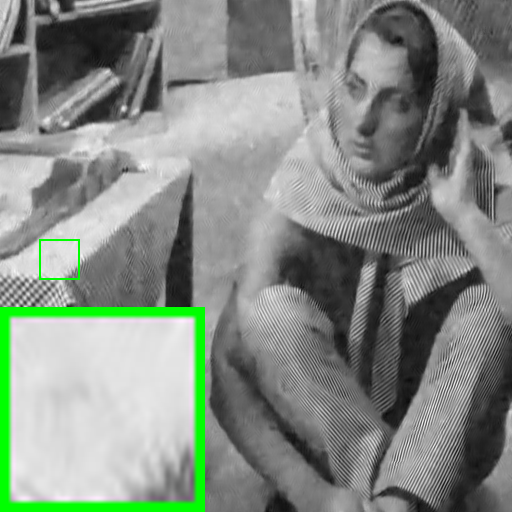
\includegraphics[width=1\textwidth]{br_barbara_BPFA_40.png}}
{\footnotesize (b) BPFA \\(27.23dB/0.7775)}
\end{minipage}
\begin{minipage}[t]{0.19\textwidth}
\centering
\raisebox{-0.15cm}{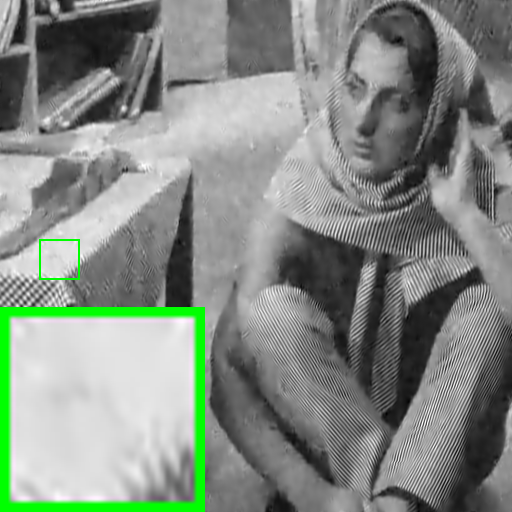
\includegraphics[width=1\textwidth]{br_barbara_BPFA_Clu_40.png}}
{\footnotesize (c) Ours: C=32,M=1\\ (27.42dB/0.7873)}
\end{minipage}
\begin{minipage}[t]{0.19\textwidth}
\centering
\raisebox{-0.15cm}{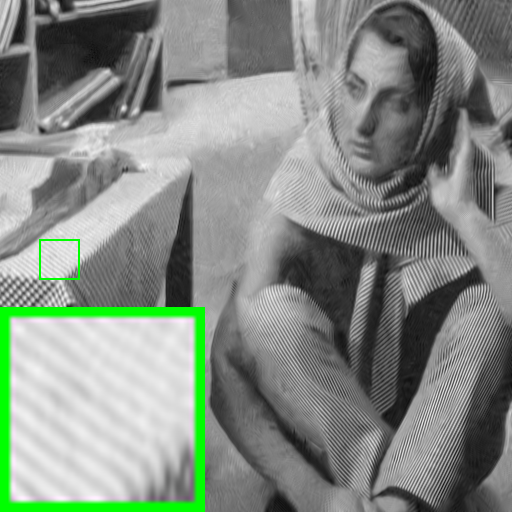
\includegraphics[width=1\textwidth]{br_barbara_BPFA_NSSDC_40.png}}
{\footnotesize (d) Ours: C=1,M=6\\ (28.00dB/0.8072)}
\end{minipage}
\begin{minipage}[t]{0.19\textwidth}
\centering
\raisebox{-0.15cm}{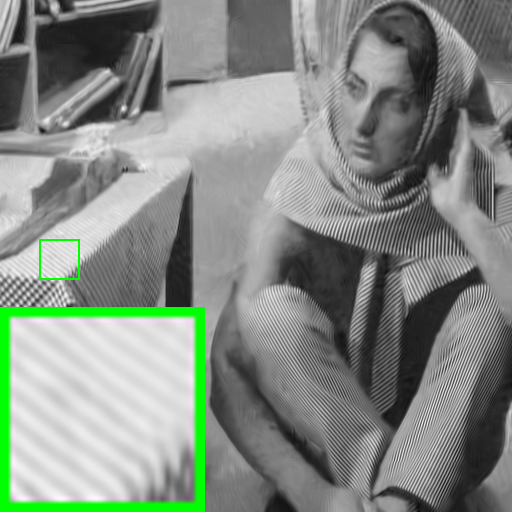
\includegraphics[width=1\textwidth]{br_barbara_BPFA_CluNSSDC_40.png}}
{\footnotesize (e) Ours: C=32,M=6 \\ (28.40dB/0.8305)}
\end{minipage}
}\vspace{-0.1in}
\caption{Denoised images of \textsl{Barbara} and PSNR/SSIM results by BPFA and our models (the standard deviation of Gaussian noise is $\sigma=40$).}
\label{fig2}
\end{figure}\vspace{-0.4in}

\subsection{PG based Bayesian Learning for Structural Clustering}
Given a noisy image, we can extracted $N$ PG variations, the $m$-th variation in the $n$-th PG is defined as
$\mathbf{\overline{x}}_{n,m}$, where $n=1,...,N$ and $m=1,...,M$. We propose to utilize Mixture of Gaussian (MoG) with $C$ components, to divide the sundry PG variations into different clusters. The relationship between PG variation $\mathbf{\overline{x}}_{n,m}$ and the MoG model relies on a latent variable defined as $\mathbf{z}_{n,m}$, which is consisted of $C$ elements $z_{n,m,c}$ for $c=1,...,C$. If PG variation $\mathbf{\overline{x}}_{n,m}$ belongs to the $c$th component, $z_{n,m,c}=1$; and otherwise $z_{n,m,c}=0$. A natural problem is how to determine $C$, the number of clusters, as well as other parameters in the MoG model. A reliable solution is to initialize $C$ as a large number and then employ the Dirichlet prior to estimate it \cite{prml}.

In order to fully estimate the parameters of the MoG model, we can resort to the posterior distribution $p(\{\mathbf{z}_{n,m}\}|\{\mathbf{\overline{x}}_{n,m}\})$ given $\{\mathbf{z}_{n,m}\}$ ($n=1,...,N$ and $m=1,...,M$). Though its analytical form is not computationally tractable, we could use variational Bayesian inference as an approximational technique. Assuming that the mixing coefficients vector is $\boldsymbol{\uppi}$, the conditional distribution of the latent variables $\{\mathbf{z}_{n,m}\}$ is 
\vspace{-0.05in}
\begin{equation}\label{equ1}
\vspace{-0.1in}
p(\{\mathbf{z}_{n,m}\}|\boldsymbol{\uppi}) = \prod_{n=1}^{N}\prod_{m=1}^{M}\prod_{c=1}^{C}\boldsymbol{\uppi}_{c}^{z_{n,m,c}}.
\end{equation}
The conditional distribution of the PG variations is 
\vspace{-0.1in}
\begin{equation}\label{equ2}
\vspace{-0.1in}
p(\{\mathbf{\overline{x}}_{n,m}\}|\{\mathbf{z}_{n,m}\},\{\boldsymbol{\upmu}_{c}\},\{\mathbf{\Sigma}_{c}\}) = \prod_{n=1}^{N}\prod_{m=1}^{M}\prod_{c=1}^{C}\mathcal{N}(\mathbf{\overline{x}}_{n,m}|\boldsymbol{\upmu}_{c},\mathbf{\Sigma}_{c})^{z_{n,m,c}}
\end{equation}
where $\boldsymbol{\upmu}_{c}$ and $\mathbf{\Sigma}_{c}$ are the corresponding mean vector and covariance matrix of the $c$-th component of the MoG model. After introducing corresponding priors over the parameters $\{\mathbf{z}_{n,m}\}$, $\{\boldsymbol{\upmu}_{c}\}$ and $\{\mathbf{\Sigma}_{c}\}$, we can write the joint distribution of all the variables by 
\vspace{-0.05in}
\begin{equation}\label{equ3}
\vspace{-0.05in}
\begin{split}
&p(\{\mathbf{\overline{x}}_{n,m}\},\{\mathbf{z}_{n,m}\},\boldsymbol{\uppi},\{\boldsymbol{\upmu}_{c}\},\{\mathbf{\Sigma}_{c}\}) 
=
p(\{\mathbf{\overline{x}}_{n,m}\}|\{\mathbf{z}_{n,m}\},\{\boldsymbol{\upmu}_{c}\},
\\
&
\{\mathbf{\Sigma}_{c}\})\times p(\{\mathbf{z}_{n,m}\}|\boldsymbol{\uppi})
\times p(\boldsymbol{\uppi})
\times p(\boldsymbol{\upmu}_{c}|\mathbf{\Sigma}_{c})
\times p(\{\mathbf{\Sigma}_{c}\}),
\end{split}
\end{equation}
where the mixing coefficients vector $\boldsymbol{\uppi}$ is assumed to follow Dirichlet distribution.

Finally, we can perform variational maximization (M step) and expectation estimatation of the responsibilities (E step) alternatively. By taking suitable parameters for the equation \ref{equ3}, we can re-write the lower bound as a function of the parameters. This lower bound can be used to determine the posterior distribution over the number of components $C$ in the MoG model. Please refer to \cite{prml} for more details. We use the Matlab code implemented in Pattern Recognition and Machine Learning Toolbox \url{http://www.mathworks.com/matlabcentral/fileexchange/55826-pattern-recognition-and-machine-learning-toolbox}.
\vspace{-0.1in}

\subsection{Discussion}
Based on above description, we discuss as follows the advantages of the proposed model for PG based modeling directly on noisy images: Firstly, all the parameters of the proposed model are automatically estimated from the noisy image via variational Bayesian inference. This is a major advantage over PGPD \cite{pgpd}. Secondly, we demonstrated that structural clustering can indeed boost the performance of Bayesian methods such as BPFA \cite{bpfa}. This is demonstrated in the images (b) and (c) of Figure \ref{fig2}. Thirdly, the Non-local Self Similarity prior can be used to improve the performance of BPFA \cite{bpfa}. This can be demonstrated by comparing the images ((b), (c), (e)) or ((b), (d), (e)).
\vspace{-0.1in}

\section{Patch Group based Bayesian Dictionary Learning}
\subsection{Truncated beta-Bernoulli Process for Dictionary Learning}
\vspace{-0.1in}
Once we have clustered similar PG variations into different components, we can extract the latent clean PG variations using sparse or low rank image priors. These priors are also frequently employed by many state-of-the-art methods \cite{bm3d,lssc,epll,ncsr,wnnm,pgpd} for image restoration tasks. We do not fixed the number of atoms in the dictionary learning. This is different from the previous methods, including PGPD. Instead, we set a large number $K$, which makes our Bayesian model a truncated beta-Bernoulli process. We employ the beta-Bernoulli process \cite{hjort1990,thibaux2007,paisley2009} to seek the sparse priors on infinite feature space.

In this paper, we express noisy PG variations $\mathbf{\overline{X}}$ as\vspace{-0.1in}
\begin{equation}\label{equ7}
\mathbf{\overline{X}} = \mathbf{D}\mathbf{W}+\mathbf{V},\vspace{-0.1in}
\end{equation}
where $\mathbf{\overline{X}}\in\mathbb{R}^{p^2\times M}$, the coefficients vector 
$\mathbf{W}\in\mathbb{R}^{K\times M}$, and the noise term $\mathbf{V} \in \mathbb{R}^{p^2\times M}$. The matrix $\mathbf{D}\in \mathbb{R}^{p^2\times K}$ contains $K$ dictionary atoms. The coefficients matrix $\mathbf{W}$ is represented by $\mathbf{W} = \mathbf{B}\odot\mathbf{S}$. The matrices $\mathbf{B}, \mathbf{S}\in\mathbb{R}^{K\times M}$ are the binary matrix and the coefficients matrix, respectively and $\odot$ is the element-wise product. We denote $\mathbf{\overline{x}}$ as any column of the PG variations $\mathbf{\overline{X}}$ and $\mathbf{w}, \mathbf{b}\in\{0,1\}^{K}$, and $\mathbf{s}$ as corresponding columns of the coefficients matrix $\mathbf{W}$, the binary matrix $\mathbf{B}$, and the coefficients matrix $\mathbf{S}$. We denote $\{\mathbf{d}_{k}\}_{j=1}^{K}$ as columns of the dictionary $\mathbf{D}$, $\{\mathbf{s}_{j}\}_{j=1}^{n}$ as columns of $\mathbf{S}$, and $\{\mathbf{v}_{j}\}_{j=1}^{n}$ as columns of the noise matrix $\mathbf{V}$. Each column $\mathbf{w}$ is represented by a binary vector $\mathbf{b}\in\{0,1\}^{K}$ and a coefficient vector $\mathbf{s}\in\mathbb{R}^{K\times 1}$, i.e., $\mathbf{w} = \mathbf{b}\odot\mathbf{s}$. Then we can impose suitable priors on these parameters, i.e., $\mathbf{b}$, $\{\mathbf{d}_{k}\}_{k=1}^{K}$, $\{\mathbf{s}_{k}\}_{k=1}^{K}$, and $\{\mathbf{v}_{j}\}_{j=1}^{n}$. The binary vector $\mathbf{b}\in\{0,1\}^{K}$ denotes which of the columns (or atoms) in $\mathbf{D}$ are used for the representation of $\mathbf{\overline{x}}$. At beginning, we do not know the suitable $K$. We can set $K \rightarrow \infty$ and impose sparse prior on $\mathbf{b}\in\{0,1\}^{K}$ to limit the number of atoms in $\mathbf{D}$ used for representing each PG variation $\mathbf{\overline{x}}$ extracted from noisy images. The beta-Bernoulli process \cite{hjort1990,thibaux2007,paisley2009} provides a convenient way for this purpose. For inference convenience, we impose independent Gaussian priors on $\{\mathbf{d}_{k}\}_{k=1}^{K}$, $\{\mathbf{s}_{k}\}_{k=1}^{K}$, and $\{\mathbf{v}_{j}\}_{j=1}^{n}$.

The dictionary learning model for PG variations is 
\vspace{-0.1in}
\begin{equation}\label{equ8}\vspace{-0.1in}
\mathbf{\overline{X}} = \mathbf{D}\mathbf{W}+\mathbf{V}, \mathbf{W} = \mathbf{B}\odot\mathbf{S},
\end{equation}
where $\odot$ is element-wise product.
The beta-Bernoulli process \cite{paisley2009} for binary vector is:
\vspace{-0.1in}
\begin{equation}\label{equ9}
\mathbf{b} \sim \prod_{k=1}^{K}Bernoulli(\pi_{k}), \boldsymbol{\pi}\sim\prod_{k=1}^{K}Beta(\frac{a}{K},\frac{b(K-1)}{K}),
\vspace{-0.1in}
\end{equation}
\begin{equation}\label{equ10}
\mathbf{d}_{k}\sim\mathcal{N}(0,P^{-1}\mathbf{I}_{P}), 
\mathbf{s}_{j} \sim \mathcal{N}(0,\gamma_{s}^{-1}\mathbf{I}_{K}), 
\mathbf{v}_{j}\sim\mathcal{N}(0,\gamma_{v}^{-1}\mathbf{I}_{P}),
\vspace{-0.05in}
\end{equation}
\begin{equation}\label{equ11}
\gamma_{s}\sim Gamma(c,d), \gamma_{v}\sim Gamma(e,f),
\vspace{-0.05in}
\end{equation}
where $\{a,b\},\{c,d\},\{e,f\}$ are the corresponding hyper parameters of the parameters $\boldsymbol{\pi}$, $\gamma_{s}$, and $\gamma_{v}$ in the conjugate hyper priors in equations (\ref{equ9}), (\ref{equ11}). The inference procedures we take for the Bayesian model is Gibbs sampling \cite{bpfa2012} and we ignore the procedures here. As we can see, the noise estimation is integrated into the overall model in Gibbs samppling process. That is th reason why the proposed algorithm can be used to deal with blind noise. This is also different from the other non-blind image denoising methods \cite{nlm,bm3d,lssc,epll,ncsr,wnnm,pgpd}, since they do not have the ability to estimate the noise within the noisy images.

We compare the proposed model with the BPFA model on the dictionary elements. With the help of PG based NSS prior and structural clustering, the dictionary learned by the proposed model is more representative and discriminative than that learned by the BPFA model \cite{bpfa}. Take the image "Barbara" for an example, it is corrupted by Gaussian noise with $\sigma = 40$. The initial number of dictionary elements is $512$ for both methods. In Figure \ref{fig2} (a), we demonstrate the dictionary elements learned by the BPFA model \cite{bpfa}. In the (b), (c), and (d) of Figure \ref{fig2}, we demonstrate the dictionary elements of three components learned by the proposed method. Noted that the BPFA learned from the original patches while the proposed method learned from patch group variations. It can be seen that these dictionary elements express the latent clean structures of the noisy PG variations in this component. For different Gaussian components, we can see that the number of elements are automatically determined by the nonparametric Bayesian inference. The dictionary elements in the subfigures (a) to (d) in Figure \ref{fig3} are supplemented by black patches to make sure that these subfigures are square.
\vspace{-0.2in}
\begin{figure}
\centering
\subfigure{
\begin{minipage}{0.24\textwidth}
\centering
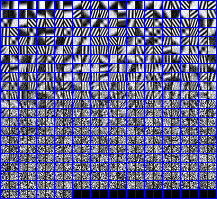
\includegraphics[width=1\textwidth]{BPFA_barbara_40_dict.png}
{\footnotesize (a)}
\end{minipage}
\begin{minipage}{0.24\textwidth}
\centering
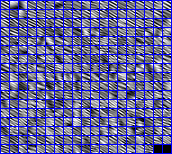
\includegraphics[width=1\textwidth]{barbara_Iteration8_dict2.png}
{\footnotesize (b)}
\end{minipage}
\begin{minipage}{0.24\textwidth}
\centering
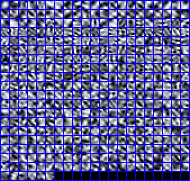
\includegraphics[width=1\textwidth]{barbara_Iteration8_dict3.png}
{\footnotesize (c)}
\end{minipage}
\begin{minipage}{0.24\textwidth}
\centering
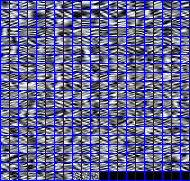
\includegraphics[width=1\textwidth]{barbara_Iteration8_dict4.png}
{\footnotesize (d)}
\end{minipage}
}\vspace{-0.15in}
\caption{The dictionary elements learned by the BPFA model ((a)) and the proposed method ((b), (c), and (d)).}
\label{fig3}
\end{figure}

\subsection{Discussion}
Our method are different from the method of BPFA \cite{bpfa}. Basicly, our model learns flexible number of dictionary atoms on patch groups while BPFA fixs the number of dictioary atoms learned over patches. This modification makes the dictionary more representative and discriminative than those in BPFA \cite{bpfa}. What's more, BPFA is only applied in (non-blind) denoising Gaussian noise while our model is applied to (blind) denoising multiple noises such as Gaussian noise, mixed Gaussian and impulse noise, and real noise. This will be demonstrated in the experimental section.

\section{Summary of The Overall Algorithm}
The overall algorithm is consisted of three parts. The first is the PG based Bayesian learning for automatically estimating the parameters of the MoG model, including the number of components. After the clustering, we employ a divide-and-conquer strategy. The second part is, for each component, we employ the PG based nonparametric Bayesian dictionary learning to sample the dictionary $\mathbf{D}$ as well as coefficients matrix $\mathbf{W}$. Then, the final denoised PG variations is simply calculated as $\hat{\mathbf{X}} = \mathbf{D}\mathbf{W}$. That is the key factor why the proposed algorithm is able to deal with blind image denoising. After this is done for each component, the third part is to recover the denoised image by aggregating the denoised PGs. The overall algorithm is summarized in Algorithm 1. The Matlab source code of our algorithm can be downloaded at \url{http://www4.comp.polyu.edu.hk/~csjunxu/code/PGBL_BID.zip}.
\begin{table}[t]
\centering
\label{alg}
\begin{tabular}{l}
\hline
\textbf{Algorithm 1}: The Overall Algorithm
\\
\hline
\textbf{Input:} Noisy image $\mathbf{y}, a=b=1,c=d=e=f=10^{-6}$
\\
\ 1. Extract non-local similar patch groups $\{\mathbf{X}\}$;
\\
\ 2. For each PG, calculate its mean $\boldsymbol{\upmu}_{x}$ and form PG variations $\mathbf{\overline{X}}$;
\\
\ 3. Estimate the parameters in MoG model via variational Bayesian inference;
\\
\ 4.\quad \textbf{for} each cluster
\\
\ 5.\quad\quad \textbf{for} $t = 1:IteNum$ \textbf{do} Gibbs Sampling:
\\
\ 6.\quad\quad\quad\ Sample $\mathbf{b}$ from equation (\ref{equ9})
\\
\ 7.\quad\quad\quad\ Sample $\mathbf{d}_{k}\sim\mathcal{N}(0,P^{-1}\mathbf{I}_{P})$
\\
\ 8.\quad\quad\quad\ Sample $\mathbf{s}_{j} \sim \mathcal{N}(0,\gamma_{s}^{-1}\mathbf{I}_{K}, \gamma_{s}\sim Gamma(c,d)$
\\
\ 9.\quad\quad\quad\ Sample $\mathbf{v}_{j}\sim\mathcal{N}(0,\gamma_{v}^{-1}\mathbf{I}_{P}), \gamma_{v}\sim Gamma(e,f)$
\\
10.\quad\quad\textbf{end for}
\\
11.\quad Recover each patch group via $\hat{\mathbf{X}}=\mathbf{D}\mathbf{W}+\boldsymbol{\upmu}_{x}$;
\\
12.\quad \textbf{end for}
\\
13. Average the recovered patch groups to form the recovered image $\hat{\mathbf{y}}$;
\\
14. \textbf{Output:} The recovered image $\hat{\mathbf{y}}$.\\
\hline
\end{tabular}
\end{table}

\vspace{-0.1in}

%------------------------------------------------------------------------- 
\section{Experiments}
\begin{figure*}[t]
\centering
\subfigure{
\begin{minipage}{0.09\textwidth}
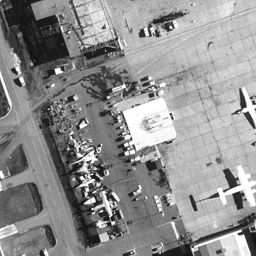
\includegraphics[width=1.06\textwidth]{airfield.png}
\end{minipage}
\begin{minipage}{0.09\textwidth}
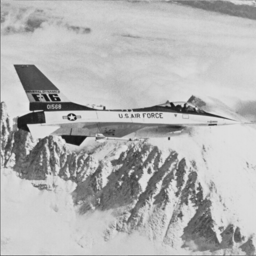
\includegraphics[width=1.06\textwidth]{airplane.png}
\end{minipage}
\begin{minipage}{0.09\textwidth}
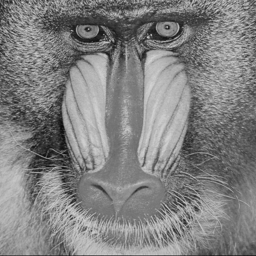
\includegraphics[width=1.06\textwidth]{baboon.png}
\end{minipage}
\begin{minipage}{0.09\textwidth}
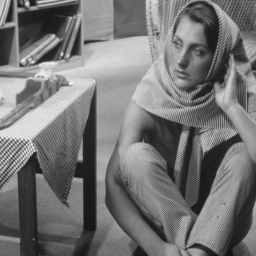
\includegraphics[width=1.06\textwidth]{barbara.png}
\end{minipage}
\begin{minipage}{0.09\textwidth}
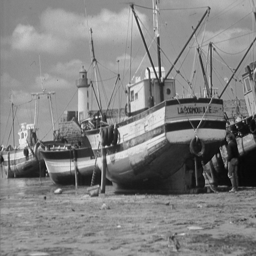
\includegraphics[width=1.06\textwidth]{boat.png}
\end{minipage}
\begin{minipage}{0.09\textwidth}
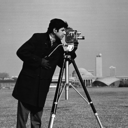
\includegraphics[width=1.06\textwidth]{cameraman.png}
\end{minipage}
\begin{minipage}{0.09\textwidth}
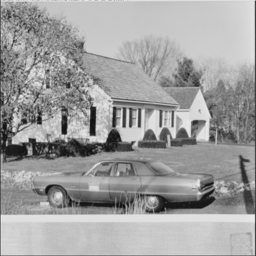
\includegraphics[width=1.06\textwidth]{carhouse.png}
\end{minipage}
\begin{minipage}{0.09\textwidth}
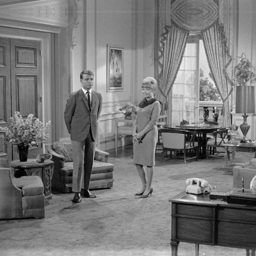
\includegraphics[width=1.06\textwidth]{couple.png}
\end{minipage}
\begin{minipage}{0.09\textwidth}
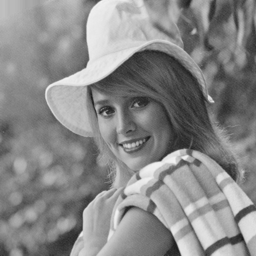
\includegraphics[width=1.06\textwidth]{elaine.png}
\end{minipage}
\begin{minipage}{0.09\textwidth}
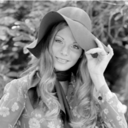
\includegraphics[width=1.06\textwidth]{hat.png}
\end{minipage}
}\vspace{-0.05in}
\setlength{\floatsep}{5pt plus 1.0pt minus 2.0pt}
\subfigure{
\begin{minipage}{0.09\textwidth}
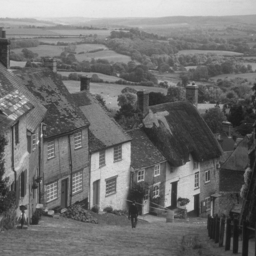
\includegraphics[width=1.06\textwidth]{hill.png}
\end{minipage}
\begin{minipage}{0.09\textwidth}
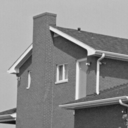
\includegraphics[width=1.06\textwidth]{house.png}
\end{minipage}
\begin{minipage}{0.09\textwidth}
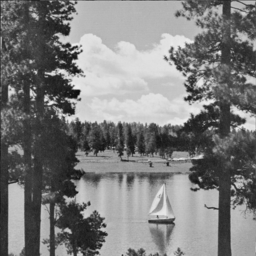
\includegraphics[width=1.06\textwidth]{lake.png}
\end{minipage}
\begin{minipage}{0.09\textwidth}
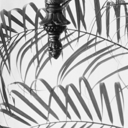
\includegraphics[width=1.06\textwidth]{leaves.png}
\end{minipage}
\begin{minipage}{0.09\textwidth}
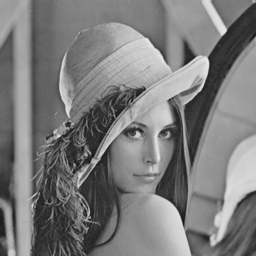
\includegraphics[width=1.06\textwidth]{lena.png}
\end{minipage}
\begin{minipage}{0.09\textwidth}
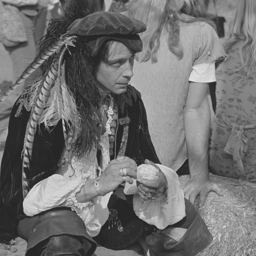
\includegraphics[width=1.06\textwidth]{man.png}
\end{minipage}
\begin{minipage}{0.09\textwidth}
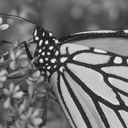
\includegraphics[width=1.06\textwidth]{monarch.png}
\end{minipage}
\begin{minipage}{0.09\textwidth}
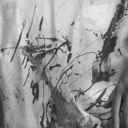
\includegraphics[width=1.06\textwidth]{paint.png}
\end{minipage}
\begin{minipage}{0.09\textwidth}
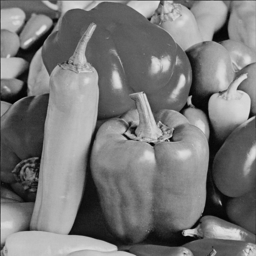
\includegraphics[width=1.06\textwidth]{peppers.png}
\end{minipage}
\begin{minipage}{0.09\textwidth}
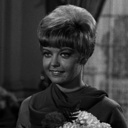
\includegraphics[width=1.06\textwidth]{zelda.png}
\end{minipage}
}\vspace{-0.1in}
\caption{The 20 widely used test images.}
\label{fig4}\vspace{-0.2in}
\end{figure*}
In this section, we perform image denoising experiments on various types of noise, including synthetic noise and real noise in real world images. The synthetic noise includes additive white Gaussian noise (AWGN), mixed Gaussian and random value impulse noise (RVIN). The synthetic image denoising experiments are performed on 20 widely used natural images listed in Figure \ref{fig4}. In the synthetic noise removal experiments, we compare the proposed method with other state-of-the-art methods such as \cite{bpfa,bm3d,pgpd,wnnm,cai2010fast,wesnr,noiseclinic}. The BPFA \cite{bpfa} BM3D \cite{bm3d}, PGPD \cite{pgpd}, and WNNM \cite{wnnm} are designed especially for Gaussian noise removal. The Two Phase \cite{cai2010fast} and WESNR \cite{wesnr} are designed especially for mixed Gaussian and impulse noise removal. The "Noise Clinic" method \cite{noiseclinic} is designed especially for real noise removal. It is a state-of-the-art blind denoising method. We evaluate all these methods on PSNR, SSIM \cite{ssim}, and visual quality. On real noise removal, besides the above methods, we also compare with the commercial software Neat Image \cite{neatimage}. This software is embeded in Photoshop CS, a famous commercial software for image processing. The codes or executive package of these methods are provided on the corresponding websites. Since there is no ground truth in real noise removal, we only compare the visual quality of the recovered images by these methods.

\vspace{-0.15in}

\subsection{Implementation Details}
For the BM3D \cite{bm3d}, WNNM \cite{wnnm}, and PGPD \cite{pgpd}, the input standard derivation of the noise is a key parameter. We employ a robust noise estimation method \cite{liu2013single} to estimate the noise standard derivation for these methods. The methods Two Phase \cite{cai2010fast} and WESNR \cite{wesnr} do not need the noise level as input when performing denoising tasks. But they need some preprocessing for the noise removal tasks. However, our proposed method doesn't need noise estimation nor image preprocessing.

In the proposed method, we set the initial number of components $C$ as 32. The final number of components will be automatically determined by variational Bayesian inference introduced in section 2. The patch size is fixed as $8 \times 8$, so the dimension of each patch vector is 64. The number of dictionary atoms $K$ is set to be 256 when number of PG variations in this component is less than $10^4$, otherwise the number is set to 512. The hyperparameters are fixed as $a=b=1$, $c=d=e=f=10^{-6}$ in all the experiments. We do not tune these paramters in our experiments. The number of patches in a group is set to 6. We set the maximal iteration number as 10. The $IteNum$ is set as 50. The proposed algorithm will be terminated when the noise variance of each component is less than or equal to 1.

\vspace{-0.1in}

\subsection{Additive White Gaussian Noise Removal}
Here, we compare the proposed method on Gaussian noise removal with other competing methods: BPFA \cite{bpfa}, BM3D \cite{bm3d}, and PGPD \cite{pgpd}, WNNM \cite{wnnm}, Two Phase \cite{cai2010fast}, WNSER \cite{wesnr}, Noise Clinic \cite{noiseclinic}. As a common experimental setting, we add additive white Gaussian noise with zero mean and standard deviation $\sigma$ to the test images. The denoising experiments are performed on multiple noise levels of $\sigma = 30, 40, 50, 75$.

The averaged results on PSNR and SSIM are listed in Tables \ref{tab1} and \ref{tab2}. We can see that the PSNR and SSIM results of our proposed method are much better than the BPFA, Two Phase, and WESNR, Noise Clinic methods. The results of the proposed method are comparable to BM3D when the noise levels are higher than 30. Though getting inferior results on PSNR and SSIM when compared to WNNM and PGPD, the proposed method can achieve similar or even better performance when compared with other methods. For instance, from Figure \ref{fig4} and Figure \ref{fig5}, we can see that the proposed method generates better image quality and less artifacts on the image "House" and "Hill" than the other methods. Considering that the proposed method is fully blind, it is more convincing to see that our proposed method achieves better image quality results than the Noise Clinic \cite{noiseclinic}, which is a state-of-the-art blind image denoising method. We want to mention again that BM3D, PGPD, and WNNM can only work well on the Gaussian noise, which they are designed for, but perform poorly on other types of noise, which will be demonstrated later. 
\vspace{-0.1in}
\begin{table*}
\caption{Average PSNR(dB) results of different algorithms on 20 natural images corrupted by Gaussian noise.}
\vspace{-0.1in}
\label{tab1}
\begin{center}
\renewcommand\arraystretch{1}
\small
\begin{tabular}{|c||c|c|c|c|c|c|c|c|}
\hline
$\sigma$ & \textbf{BPFA} &\textbf{BM3D}&\textbf{WNNM}& \textbf{PGPD} &\textbf{Two Phase} & \textbf{WESNR} &\textbf{Noise Clinic} & \textbf{Ours}
\\
\hline
30 & 28.81 & 29.11 & 29.35 & 29.13 & 18.84 & 27.44 & 26.81 & 28.65 
\\
\hline
40 & 27.45 & 27.68 & 28.03 & 27.88 & 16.52 & 25.07 & 24.90 & 27.59 
\\
\hline
50 & 26.38 & 26.80 & 27.06 & 26.89 & 14.80 & 22.02 & 23.47 & 26.68
\\
\hline
75 & 24.40 & 25.04 & 25.25 & 25.11 & 11.95 & 9.02 & 21.31 & 24.91
\\
\hline
\end{tabular}
\end{center}
\end{table*}

\vspace{-0.3in}

\begin{table*}
\caption{Average SSIM results of different algorithms on 20 natural images corrupted by Gaussian noise.}
\vspace{-0.1in}
\label{tab2}
\begin{center}
\renewcommand\arraystretch{1}
\small
\begin{tabular}{|c||c|c|c|c|c|c|c|c|}
\hline
$\sigma$ & \textbf{BPFA} &\textbf{BM3D}&\textbf{WNNM} & \textbf{PGPD} & \textbf{Two Phase} & \textbf{WESNR} &\textbf{Noise Clinic} & \textbf{Ours}
\\
\hline
30 & 0.7988 & 0.8108 & 0.8156 &0.8089 & 0.3137 & 0.7430 & 0.6520 & 0.7971 
\\
\hline
40 & 0.7576 & 0.7706 & 0.7784 & 0.7747 & 0.2361 & 0.6063 & 0.5631 & 0.7668 
\\
\hline
50 & 0.7216 & 0.7430 & 0.7510 & 0.7435 & 0.1855 & 0.4483 & 0.4990 & 0.7382
\\
\hline
75 & 0.6470 & 0.6803 & 0.6897 & 0.6825 & 0.1147 & 0.1749 & 0.4289 & 0.6766
\\
\hline
\end{tabular}
\end{center}
\end{table*}

\begin{figure*}
\centering
\subfigure{
\begin{minipage}[t]{0.2\textwidth}
\centering
\raisebox{-0.15cm}{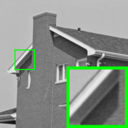
\includegraphics[width=1\textwidth]{br_Original_house.png}}
{\footnotesize (a) Ground Truth}
\end{minipage}
\begin{minipage}[t]{0.2\textwidth}
\centering
\raisebox{-0.15cm}{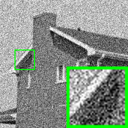
\includegraphics[width=1\textwidth]{br_Noisy_Gau_40_house.png}}
{\footnotesize (b) Noisy Image \\(16.30dB/0.1701)}
\end{minipage}
\begin{minipage}[t]{0.2\textwidth}
\centering
\raisebox{-0.15cm}{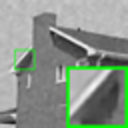
\includegraphics[width=1\textwidth]{br_BPFA_Gau_house_40.png}}
{\footnotesize (c) BPFA \\(29.75dB/0.8048)}
\end{minipage}
\begin{minipage}[t]{0.2\textwidth}
\centering
\raisebox{-0.15cm}{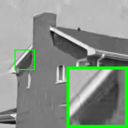
\includegraphics[width=1\textwidth]{br_BM3D_Gau_40_house.png}}
{\footnotesize (d) BM3D \\(30.63dB/0.8231)}
\end{minipage}
\begin{minipage}[t]{0.2\textwidth}
\centering
\raisebox{-0.15cm}{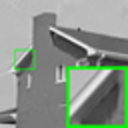
\includegraphics[width=1\textwidth]{br_PGPD_Gau_40_house.png}}
{\footnotesize (e) PGPD \\(31.02dB/0.8302)}
\end{minipage}
}
\subfigure{
\begin{minipage}[t]{0.2\textwidth}
\centering
\raisebox{-0.15cm}{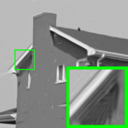
\includegraphics[width=1\textwidth]{br_WNNM_Gau_40_house.png}}
{\footnotesize (f) WNNM \\(31.19dB/0.8279)}
\end{minipage}
\begin{minipage}[t]{0.2\textwidth}
\centering
\raisebox{-0.15cm}{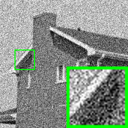
\includegraphics[width=1\textwidth]{br_TwoPhase_Gau_40_house.png}}
{\footnotesize (g) Two Phase \\(16.30dB/0.1701)}
\end{minipage}
\begin{minipage}[t]{0.2\textwidth}
\centering
\raisebox{-0.15cm}{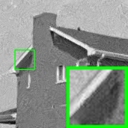
\includegraphics[width=1\textwidth]{br_WESNR_Gau_40_house.png}}
{\footnotesize (h) WESNR \\(27.27dB/0.6076)}
\end{minipage}
\begin{minipage}[t]{0.2\textwidth}
\centering
\raisebox{-0.15cm}{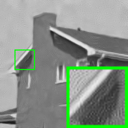
\includegraphics[width=1\textwidth]{br_NC_Gau_40_house.png}}
{\footnotesize (i) Noise Clinic \\(26.48dB/0.5370)}
\end{minipage}
\begin{minipage}[t]{0.2\textwidth}
\centering
\raisebox{-0.15cm}{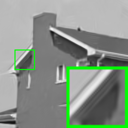
\includegraphics[width=1\textwidth]{br_Ours_Gau_40_house.png}}
{\footnotesize (j) Ours \\(30.90dB/0.8328)}
\end{minipage}
}
\vspace{-0.2in}
\caption{Denoised images of \textsl{House} and PSNR/SSIM results by different methods (the standard deviation of Gaussian noise is $\sigma=40$).}
\label{fig5}
\end{figure*}\vspace{-0.3in}

\begin{figure*}
\centering
\subfigure{
\begin{minipage}[t]{0.2\textwidth}
\centering
\raisebox{-0.15cm}{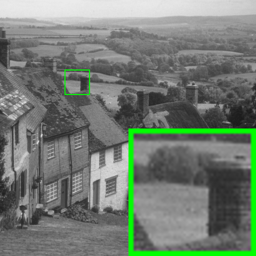
\includegraphics[width=1\textwidth]{br_Original_hill.png}}
{\footnotesize (a) Ground Truth}
\end{minipage}
\begin{minipage}[t]{0.2\textwidth}
\centering
\raisebox{-0.15cm}{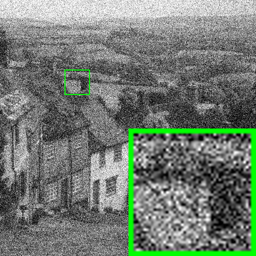
\includegraphics[width=1\textwidth]{br_Noisy_Gau_50_hill.png}}
{\footnotesize (b) Noisy Image \\(14.68dB/0.1357)}
\end{minipage}
\begin{minipage}[t]{0.2\textwidth}
\centering
\raisebox{-0.15cm}{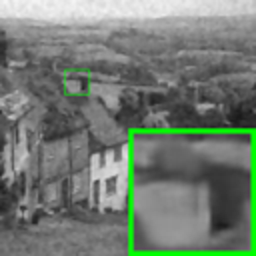
\includegraphics[width=1\textwidth]{br_BPFA_Gau_hill_50.png}}
{\footnotesize (c) BPFA \\(26.81dB/0.6530)}
\end{minipage}
\begin{minipage}[t]{0.2\textwidth}
\centering
\raisebox{-0.15cm}{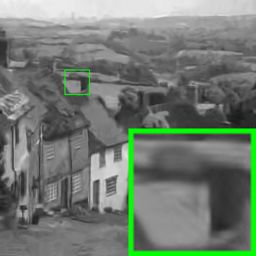
\includegraphics[width=1\textwidth]{br_BM3D_Gau_50_hill.png}}
{\footnotesize (d) BM3D \\(27.19dB/0.6745)}
\end{minipage}
\begin{minipage}[t]{0.2\textwidth}
\centering
\raisebox{-0.15cm}{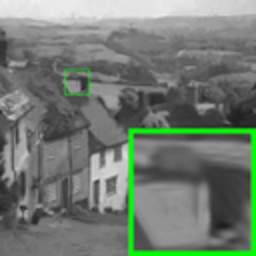
\includegraphics[width=1\textwidth]{br_PGPD_Gau_50_hill.png}}
{\footnotesize (e) PGPD \\(27.22dB/0.6702)}
\end{minipage}
}
\subfigure{
\begin{minipage}[t]{0.2\textwidth}
\centering
\raisebox{-0.15cm}{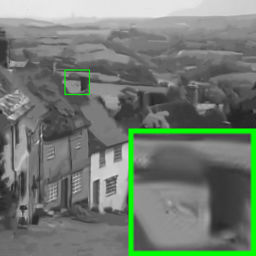
\includegraphics[width=1\textwidth]{br_WNNM_Gau_50_hill.png}}
{\footnotesize (f) WNNM \\(27.34dB/0.6772)}
\end{minipage}
\begin{minipage}[t]{0.2\textwidth}
\centering
\raisebox{-0.15cm}{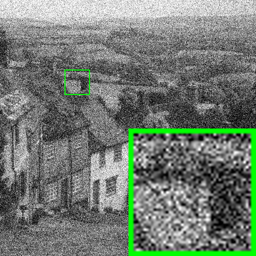
\includegraphics[width=1\textwidth]{br_TwoPhase_Gau_50_hill.png}}
{\footnotesize (g) Two Phase \\(14.68dB/0.1357)}
\end{minipage}
\begin{minipage}[t]{0.2\textwidth}
\centering
\raisebox{-0.15cm}{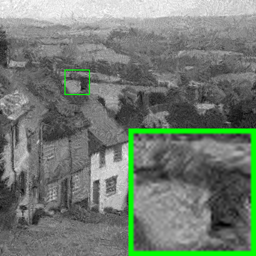
\includegraphics[width=1\textwidth]{br_WESNR_Gau_50_hill.png}}
{\footnotesize (h) WESNR \\(23.50dB/0.4218)}
\end{minipage}
\begin{minipage}[t]{0.2\textwidth}
\centering
\raisebox{-0.15cm}{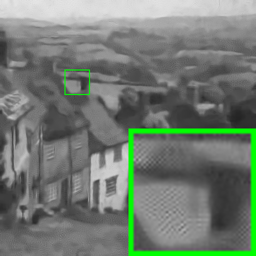
\includegraphics[width=1\textwidth]{br_NC_Gau_50_hill.png}}
{\footnotesize (i) Noise Clinic \\(25.01dB/0.5128)}
\end{minipage}
\begin{minipage}[t]{0.2\textwidth}
\centering
\raisebox{-0.15cm}{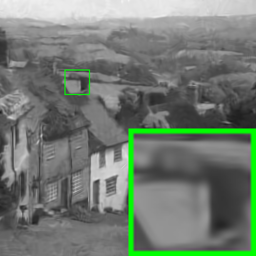
\includegraphics[width=1\textwidth]{br_Ours_Gau_50_hill.png}}
{\footnotesize (j) Ours \\(27.02dB/0.6618)}
\end{minipage}
}
\vspace{-0.1in}
\caption{Denoised images of \textsl{Hill} and PSNR/SSIM results by different methods (the standard deviation of Gaussian noise is $\sigma=50$).}
\label{fig6}
\end{figure*}

\subsection{Mixed Gaussian and Impulse Noise Removal}
Here, we compare the proposed method on mixed Gaussian and impulse noise with the compared methods \cite{bpfa,bm3d,pgpd,wnnm,cai2010fast,wesnr,noiseclinic}. We consider Random Value Impulse Noise (RVIN) here. The pixels in the testing image corrupted by RVIN is distributed between 0 and 255. This is much harder than salt and pepper noise, which is only 0 or 255 values. In the synthetic noise, the standard derivations of the Gaussian noise are $\sigma=10, 20$ and the ratios of the impulse noise are $0.15, 0.30$, respectively. The RVIN noise is generated by the "impulsenoise" function used by WESNR \cite{wesnr}. 

For BPFA \cite{bpfa}, BM3D \cite{bm3d}, and PGPD \cite{pgpd}, WNNM \cite{wnnm}, they are designed to deal with Gaussian noise. Hence, we still employ the noise estimation method \cite{liu2013single} to estimate the noise levels $\sigma$. We also compare the proposed method with the methods Two Phase \cite{cai2010fast} and WESNR \cite{wesnr}, which are designed especially for the mixed Gaussian and RVIN noise. Noted that both Two Phase \cite{cai2010fast} and WESNR \cite{wesnr} employ Adaptive Median Filter (AMF) \cite{amf} to preprocess the image before performing image denoising task. We also compare with the Noise Clinic \cite{noiseclinic}.

The results on PSNR and SSIM are listed in Table \ref{tab3} and Table \ref{tab4}. As we can see, the performance of the proposed method is comparable or better than other methods. For the visual quality comparison, the proposed method can generate better results than other methods. Take the image "Couple" for an example, from the Figure \ref{fig7}, the proposed method removes the noise clearly while all other methods remain some noise or generate some artifacts. From the results on "Barbara" listed in Figure \ref{fig8}, the proposed method achieves higher SSIM and generates better image quality than all other methods. We have to mention again that the Two Phase and WESNR are two state-of-the-art methods designed especially for the mixed Gaussian and impulse noise. But they perform poorly on other types of noises such as Gaussian.
\vspace{-0.05in}
\begin{table*}
\vspace{-0.1in}
\caption{Average PSNR(dB) results of different algorithms on 20 natural images corrupted by mixed of Gaussian and RVIN noise.}
\vspace{-0.1in}
\label{tab3}
\begin{center}
\renewcommand\arraystretch{1}
\footnotesize
\begin{tabular}{|c||c|c|c|c|c|c|c|c|}
\hline
$\sigma$, \text{Ratio}& \textbf{BPFA} &\textbf{BM3D}&\textbf{WNNM}&\textbf{PGPD}&\textbf{Two Phase}& \textbf{WESNR}& \textbf{Noise Clinic}&\textbf{Ours}
\\
\hline
$10, 0.15$ &  17.12  &  25.18   & 22.98  & 25.41 &   27.28     &   27.37   &  18.66   & 27.17
\\
\hline
$10, 0.30$& 14.19  &  21.80   & 21.40 & 21.74  &   26.12    &  21.50        &   16.44  & 22.17
\\
\hline
$20, 0.15$& 17.62  &  25.13   & 23.57 & 25.33  & 24.43     &   27.24      &  19.66   & 26.12
\\
\hline
$20, 0.30$& 17.61  & 21.73    & 21.40 & 21.64  & 23.61    & 22.69      &  14.46   & 21.89
\\
\hline
\end{tabular}
\end{center}
\end{table*}
\vspace{-0.5in}

\begin{table*}
\vspace{-0.1in}
\caption{Average SSIM results of different algorithms on 20 natural images corrupted by mixed of Gaussian and RVIN noise.}
\vspace{-0.1in}
\label{tab4}
\begin{center}
\renewcommand\arraystretch{1}
\footnotesize
\begin{tabular}{|c||c|c|c|c|c|c|c|c|}
\hline
$\sigma$, \text{Ratio}& \textbf{BPFA} &\textbf{BM3D}&\textbf{WNNM}&\textbf{PGPD}&\textbf{Two Phase}& \textbf{WESNR}& \textbf{Noise Clinic}&\textbf{Ours}
\\
\hline
$10, 0.15$& 0.2749 & 0.7037    & 0.5806 & 0.7242  &   0.7091  &  0.7499      &  0.3198   & 0.7459
\\
\hline
$10, 0.30$& 0.1576  & 0.6444    & 0.6038 & 0.6405  &  0.6783     &  0.4970     &  0.2042   & 0.6559
\\
\hline
$20, 0.15$& 0.2821  &  0.7132   & 0.6190 & 0.7220  &   0.5468    &   0.7568     & 0.3423    & 0.7312
\\
\hline
$20, 0.30$& 0.2821  & 0.6414    & 0.6310 & 0.6371  &   0.5183   &   0.5871     &  0.1346   & 0.6470
\\
\hline
\end{tabular}
\end{center}\vspace{-0.4in}
\end{table*}

\begin{figure*}
\centering
\subfigure{
\begin{minipage}[t]{0.2\textwidth}
\centering
\raisebox{-0.15cm}{\includegraphics[width=1\textwidth]{br_Original_couple.png}}
{\footnotesize (a) Ground Truth}
\end{minipage}
\begin{minipage}[t]{0.2\textwidth}
\centering
\raisebox{-0.15cm}{\includegraphics[width=1\textwidth]{br_Noisy_GauRVIN_10_015_couple.png}}
{\footnotesize (b) Noisy Image \\(17.35dB/0.2852)}
\end{minipage}
\begin{minipage}[t]{0.2\textwidth}
\centering
\raisebox{-0.15cm}{\includegraphics[width=1\textwidth]{br_BPFA_GauRVIN_10_015_couple.png}}
{\footnotesize (c) BPFA \\(17.80dB/0.2871)}
\end{minipage}
\begin{minipage}[t]{0.2\textwidth}
\centering
\raisebox{-0.15cm}{\includegraphics[width=1\textwidth]{br_BM3D_GauRVIN_10_015_couple.png}}
{\footnotesize (d) BM3D \\(25.70dB/0.7126)}
\end{minipage}
\begin{minipage}[t]{0.2\textwidth}
\centering
\raisebox{-0.15cm}{\includegraphics[width=1\textwidth]{br_PGPD_GauRVIN_10_015_couple.png}}
{\footnotesize (e) PGPD \\(25.75dB/0.7208)}
\end{minipage}
}
\subfigure{
\begin{minipage}[t]{0.2\textwidth}
\centering
\raisebox{-0.15cm}{\includegraphics[width=1\textwidth]{br_WNNM_GauRVIN_10_015_couple.png}}
{\footnotesize (f) WNNM \\(23.81dB/0.6162)}
\end{minipage}
\begin{minipage}[t]{0.2\textwidth}
\centering
\raisebox{-0.15cm}{\includegraphics[width=1\textwidth]{br_TwoPhase_GauRVIN_10_015_couple.png}}
{\footnotesize (g) Two Phase \\(27.47dB/0.7186)}
\end{minipage}
\begin{minipage}[t]{0.2\textwidth}
\centering
\raisebox{-0.15cm}{\includegraphics[width=1\textwidth]{br_WESNR_GauRVIN_10_015_couple.png}}
{\footnotesize (h) WESNR \\(28.40dB/0.7807)}
\end{minipage}
\begin{minipage}[t]{0.2\textwidth}
\centering
\raisebox{-0.15cm}{\includegraphics[width=1\textwidth]{br_NC_GauRVIN_10_015_couple.png}}
{\footnotesize (i) Noise Clinic \\(19.48dB/0.3378)}
\end{minipage}
\begin{minipage}[t]{0.2\textwidth}
\centering
\raisebox{-0.15cm}{\includegraphics[width=1\textwidth]{br_Ours_GauRVIN_10_015_couple.png}}
{\footnotesize (j) Ours \\(27.26dB/0.7438)}
\end{minipage}
}
\caption{Denoised images of \textsl{Couple} by different methods (the mixed Gaussian and Random Value Impulse Noise is with $\sigma = 10$ and ratio $0.15$). The images are better viewed by zooming in on screen.}
\label{fig7}
\end{figure*}

\begin{figure*}
\centering
\subfigure{
\begin{minipage}[t]{0.2\textwidth}
\centering
\raisebox{-0.15cm}{\includegraphics[width=1\textwidth]{br_Original_barbara2.png}}
{\footnotesize (a) Ground Truth}
\end{minipage}
\begin{minipage}[t]{0.2\textwidth}
\centering
\raisebox{-0.15cm}{\includegraphics[width=1\textwidth]{br_Noisy_GauRVIN_20_015_barbara.png}}
{\footnotesize (b) Noisy Image \\(16.09dB/0.2644)}
\end{minipage}
\begin{minipage}[t]{0.2\textwidth}
\centering
\raisebox{-0.15cm}{\includegraphics[width=1\textwidth]{br_BPFA_GauRVIN_20_015_barbara.png}}
{\footnotesize (c) BPFA \\(17.73dB/0.3199)}
\end{minipage}
\begin{minipage}[t]{0.2\textwidth}
\centering
\raisebox{-0.15cm}{\includegraphics[width=1\textwidth]{br_BM3D_GauRVIN_20_015_barbara.png}}
{\footnotesize (d) BM3D \\(25.58dB/0.7552)}
\end{minipage}
\begin{minipage}[t]{0.2\textwidth}
\centering
\raisebox{-0.15cm}{\includegraphics[width=1\textwidth]{br_PGPD_GauRVIN_20_015_barbara.png}}
{\footnotesize (e) PGPD \\(25.61dB/0.7633)}
\end{minipage}
}
\subfigure{
\begin{minipage}[t]{0.2\textwidth}
\centering
\raisebox{-0.15cm}{\includegraphics[width=1\textwidth]{br_WNNM_GauRVIN_20_015_barbara.png}}
{\footnotesize (f) WNNM \\(24.03dB/0.6796)}
\end{minipage}
\begin{minipage}[t]{0.2\textwidth}
\centering
\raisebox{-0.15cm}{\includegraphics[width=1\textwidth]{br_TwoPhase_GauRVIN_20_015_barbara.png}}
{\footnotesize (g) Two Phase \\(22.66dB/0.5027)}
\end{minipage}
\begin{minipage}[t]{0.2\textwidth}
\centering
\raisebox{-0.15cm}{\includegraphics[width=1\textwidth]{br_WESNR_GauRVIN_20_015_barbara.png}}
{\footnotesize (h) WESNR \\(26.74dB/0.7769)}
\end{minipage}
\begin{minipage}[t]{0.2\textwidth}
\centering
\raisebox{-0.15cm}{\includegraphics[width=1\textwidth]{br_NC_GauRVIN_20_015_barbara.png}}
{\footnotesize (i) Noise Clinic \\(19.87dB/0.3874)}
\end{minipage}
\begin{minipage}[t]{0.2\textwidth}
\centering
\raisebox{-0.15cm}{\includegraphics[width=1\textwidth]{br_Ours_GauRVIN_20_015_barbara.png}}
{\footnotesize (j) Ours \\(26.58dB/0.7853)}
\end{minipage}
}
\caption{Denoised images of \textsl{Barbara} by different methods (the mixed Gaussian and RVIN noise is with $\sigma = 20$ and ratio $0.15$). The images are better viewed by zooming in on screen.}
\label{fig8}
\end{figure*}\vspace{-0.1in}

\subsection{Real Noisy Image Denoising}
\vspace{-0.1in}
In this section, we will test the proposed method on real noise removal. Since the color images are in RGB channels, we firstly transform the color images into YCbCr channels, then perfrom denoising on the Y channel, and finally transform the denoised YCbCr channel image back into RGB channels. The denoised images are cropped to size of $800\times600$ for better visualization. We do not compare with WNNM \cite{wnnm} and Two Phase \cite{cai2010fast} here since they achieve worse denoising quality than the other methods such as BM3D \cite{bm3d}, WESNR \cite{wesnr}, and Noise Clinic \cite{noiseclinic}. For BM3D and PGPD, the input noise level $\sigma$ is still estimated by \cite{liu2013single}. We also compare with the Neat Image \cite{neatimage}, a commercial software embedded in Photoshop CS. In this paper, we take three real noisy images for examples, which are "SolvayConf1927", "Girls", and "Windmill". The image "SolvayConf1927" is an old image provided by the Noise Clinic website on IPOL \cite{ncwebsite} while the other two images are provided by the Neat Image website \cite{neatimage}. The denoised images are evaluated in Figures \ref{fig9} to \ref{fig11}.

From the results listed in Figures \ref{fig9}, \ref{fig10}, and \ref{fig11}, we can see that the proposed method can remove real noise while preserving details better than other methods. For example, in the Figure \ref{fig10}, the image "Girls" are damaged by night shot noise and hardly recoverable. However, the proposed method can denoise the heavy noise, restore the details under the noise, and make the image looks better. The details of the building in the background is zoomed in to demonstrate the advantages of our proposed method than other compared methods. Another example is the image "Windmill", the noise in night sky is traditionally difficult to remove, since it is very hard to distinct the image noise from the faint stars in the sky. Our method not only reduces the noise while generating much less artifacts, but also preserves details, i.e., the faint stars, better than other methods.
\vspace{-0.1in}
\begin{figure*}
\vspace{-0.1in}
\centering
\subfigure{
\begin{minipage}[t]{0.25\textwidth}
\centering
\raisebox{-0.15cm}{\includegraphics[width=1\textwidth]{resize_br_Real_SolvayConf1927.png}}
{\footnotesize (a) Real Noisy Image}
\end{minipage}
\begin{minipage}[t]{0.25\textwidth}
\centering
\raisebox{-0.15cm}{\includegraphics[width=1\textwidth]{resize_br_BPFA_Real_Real_SolvayConf1927.png}}
{\footnotesize (b) BPFA}
\end{minipage}
\begin{minipage}[t]{0.25\textwidth}
\centering
\raisebox{-0.15cm}{\includegraphics[width=1\textwidth]{resize_br_BM3D_Real_SolvayConf1927.png}}
{\footnotesize (c) BM3D}
\end{minipage}
\begin{minipage}[t]{0.25\textwidth}
\centering
\raisebox{-0.15cm}{\includegraphics[width=1\textwidth]{resize_br_PGPD_Real_SolvayConf1927.png}}
{\footnotesize (d) PGPD}
\end{minipage}
}
\subfigure{
\begin{minipage}[t]{0.25\textwidth}
\centering
\raisebox{-0.15cm}{\includegraphics[width=1\textwidth]{resize_br_WESNR_Real_SolvayConf1927.png}}
{\footnotesize (e) WESNR}
\end{minipage}
\begin{minipage}[t]{0.25\textwidth}
\centering
\raisebox{-0.15cm}{\includegraphics[width=1\textwidth]{resize_br_NC_Real_SolvayConf1927.png}}
{\footnotesize (f) Noise Clinic}
\end{minipage}
\begin{minipage}[t]{0.25\textwidth}
\centering
\raisebox{-0.15cm}{\includegraphics[width=1\textwidth]{resize_br_NI_Real_SolvayConf1927.png}}
{\footnotesize (g) Neat Image}
\end{minipage}
\begin{minipage}[t]{0.25\textwidth}
\centering
\raisebox{-0.15cm}{\includegraphics[width=1\textwidth]{resize_br_Ours_Real_SolvayConf1927.png}}
{\footnotesize (h) Ours }
\end{minipage}
}\vspace{-0.1in}
\caption{Denoised images of the old image "SolvayConf1927" by different methods. The images are better viewed by zooming in on screen.}
\label{fig9}\vspace{-0.4in}
\end{figure*}
  

\begin{figure*}
\centering
\subfigure{
\begin{minipage}[t]{0.25\textwidth}
\centering
\raisebox{-0.15cm}{\includegraphics[width=1\textwidth]{resize_br_Real_Niaochaogirls.png}}
{\footnotesize (a) Real Noisy Image}
\end{minipage}
\begin{minipage}[t]{0.25\textwidth}
\centering
\raisebox{-0.15cm}{\includegraphics[width=1\textwidth]{resize_br_BPFA_Real_Niaochaogirls.png}}
{\footnotesize (b) BPFA}
\end{minipage}
\begin{minipage}[t]{0.25\textwidth}
\centering
\raisebox{-0.15cm}{\includegraphics[width=1\textwidth]{resize_br_BM3D_Real_Niaochaogirls.png}}
{\footnotesize (c) BM3D}
\end{minipage}
\begin{minipage}[t]{0.25\textwidth}
\centering
\raisebox{-0.15cm}{\includegraphics[width=1\textwidth]{resize_br_PGPD_Real_Niaochaogirls.png}}
{\footnotesize (d) PGPD}
\end{minipage}
}
\subfigure{
\begin{minipage}[t]{0.25\textwidth}
\centering
\raisebox{-0.15cm}{\includegraphics[width=1\textwidth]{resize_br_WESNR_Real_Niaochaogirls.png}}
{\footnotesize (e) WESNR}
\end{minipage}
\begin{minipage}[t]{0.25\textwidth}
\centering
\raisebox{-0.15cm}{\includegraphics[width=1\textwidth]{resize_br_NC_Real_Niaochaogirls.png}}
{\footnotesize (f) Noise Clinic}
\end{minipage}
\begin{minipage}[t]{0.25\textwidth}
\centering
\raisebox{-0.15cm}{\includegraphics[width=1\textwidth]{resize_br_NI_Real_Niaochaogirls.png}}
{\footnotesize (g) Neat Image}
\end{minipage}
\begin{minipage}[t]{0.25\textwidth}
\centering
\raisebox{-0.15cm}{\includegraphics[width=1\textwidth]{resize_br_Ours_Real_Niaochaogirls.png}}
{\footnotesize (h) Ours }
\end{minipage}
}
\caption{Denoised images of the image "Girls" by different methods. The images are better viewed by zooming in on screen.}
\label{fig10}
\end{figure*}

\begin{figure*}
\centering
\subfigure{
\begin{minipage}[t]{0.25\textwidth}
\centering
\raisebox{-0.15cm}{\includegraphics[width=1\textwidth]{resize_br_Real_windmill.png}}
{\footnotesize (a) Real Noisy Image}
\end{minipage}
\begin{minipage}[t]{0.25\textwidth}
\centering
\raisebox{-0.15cm}{\includegraphics[width=1\textwidth]{resize_br_BPFA_Real_windmill.png}}
{\footnotesize (b) BPFA}
\end{minipage}
\begin{minipage}[t]{0.25\textwidth}
\centering
\raisebox{-0.15cm}{\includegraphics[width=1\textwidth]{resize_br_BM3D_Real_windmill.png}}
{\footnotesize (c) BM3D}
\end{minipage}
\begin{minipage}[t]{0.25\textwidth}
\centering
\raisebox{-0.15cm}{\includegraphics[width=1\textwidth]{resize_br_PGPD_Real_windmill.png}}
{\footnotesize (d) PGPD}
\end{minipage}
}
\subfigure{
\begin{minipage}[t]{0.25\textwidth}
\centering
\raisebox{-0.15cm}{\includegraphics[width=1\textwidth]{resize_br_WESNR_Real_windmill.png}}
{\footnotesize (c) WESNR}
\end{minipage}
\begin{minipage}[t]{0.25\textwidth}
\centering
\raisebox{-0.15cm}{\includegraphics[width=1\textwidth]{resize_br_NC_Real_windmill.png}}
{\footnotesize (d) Noise Clinic}
\end{minipage}
\begin{minipage}[t]{0.25\textwidth}
\centering
\raisebox{-0.15cm}{\includegraphics[width=1\textwidth]{resize_br_NI_Real_windmill.png}}
{\footnotesize (e) Neat Image}
\end{minipage}
\begin{minipage}[t]{0.25\textwidth}
\centering
\raisebox{-0.15cm}{\includegraphics[width=1\textwidth]{resize_br_Ours_Real_windmill.png}}
{\footnotesize (f) Ours }
\end{minipage}
}
\caption{Photo courtesy of Alexander Semenov. Denoised images of the image "Windmill" by different methods. The images are better viewed by zooming in on screen.}
\label{fig11}
\end{figure*}

\section{Conclusion}
Image denoising is a commonly encountered problem in real life. However, most denoising methods \cite{bpfa,bm3d,lssc,epll,wnnm,pgpd,cai2010fast,wesnr} need to know the noise distributions, such as Gaussian noise or mixed Gaussian and impulse noise, as well as the noise intensity. In this paper, we developed a novel blind image denoising method by patch group (PG) based nonlocal self-similarity prior modeling. We modeled the PG variations by Mixture of Gaussians \cite{prml} whose parameters, including its number of components, are inferred by variational Bayesian method. For each component, we employed nonparametric Bayesian dictionary learning \cite{bpfa,thibaux2007,paisley2009} to reconstruct the latent clean images. The proposed method can deal with unknown or arbitrary noise without knowing the noise distribution. From the experimental results on removing Gaussian noise, mixed Gaussian and random value impulse noise , and the noise in real images, we demonstrated that the proposed method achieves comparable PSNR/SSIM measurements and even better visual quality than those methods \cite{bpfa,bm3d,wnnm,pgpd,cai2010fast,wesnr,noiseclinic,neatimage}, which are specially designed for specific types of noises.



\bibliographystyle{splncs}%{ieee}%{IEEEtranS}
\bibliography{egbib}
%this would normally be the end of your paper, but you may also have an appendix
%within the given limit of number of pages
%\end{document}

%===========================================================

\end{document}
